\documentclass[uplatex,dvipdfmx,11pt]{jsarticle}
\usepackage{amsmath,amssymb,amsthm,mathtools}
\usepackage{geometry}
\usepackage{bm}
\usepackage{graphicx}
\usepackage{tikz}
\usetikzlibrary{arrows.meta,positioning}
\usepackage[unicode]{hyperref}
\providecommand{\cInv}{\cos^{-1}}
\providecommand{\E}{\mathrm{E}}
\providecommand{\V}{\mathrm{V}}
\providecommand{\Cov}{\mathrm{Cov}}
\geometry{margin=24mm}

\begin{document}
\begin{center}
{\LARGE\bfseries MORTRA 検証済み解答\par}
\vspace{1mm}
{\small 分野：解析・三角関数\qquad 問題・厳密解・図・証明経路・講評}
\end{center}
\vspace{1mm}
\hrule
\vspace{5mm}

\section*{問題}
$\displaystyle \frac{2\pi}{5}<\int_{0}^{\frac{\pi}{2}}\frac{\sin x}{x}dx<\dfrac32$ を示せ.

\section*{答え}
\(\frac{2 \pi}{5}<\displaystyle\int_0^{\pi/2}\frac{\sin x}{x}\,dx<\frac{3}{2}\)

\section*{解答}
\textbf{1.} \(0<x\le\pi/2<2\) では、正弦の交代級数の各項の絶対値は減少する。従って剰余の符号から \[1-\frac{x^2}6<\frac{\sin x}{x}<1-\frac{x^2}6+\frac{x^4}{120}\] を得る。\( x=0\) では三つとも極限値1をもつ。

\textbf{2.} これを \(0\) から \(\pi/2\) まで積分すると \[- \frac{\pi^{3}}{144} + \frac{\pi}{2}<\int_0^{\pi/2}\frac{\sin x}{x}\,dx<- \frac{\pi^{3}}{144} + \frac{\pi^{5}}{19200} + \frac{\pi}{2}.\]

\textbf{3.} 下側は \(\pi^2<10\) を用いて \[\frac{\pi}{2}-\frac{\pi^3}{144}=\pi\left(\frac12-\frac{\pi^2}{144}\right)>\frac{31\pi}{72}>\frac{2\pi}{5}.\] 上側は \(3<\pi<22/7\) と \(22^5<320\cdot7^5\) から \[\frac{\pi}{2}-\frac{\pi^3}{144}+\frac{\pi^5}{19200}<\frac{11}{7}-\frac{3}{16}+\frac{1}{60}=\frac{2353}{1680}<\frac32.\]

\textbf{4.} 以上より \[\frac{2 \pi}{5}<\int_0^{\pi/2}\frac{\sin x}{x}\,dx<\frac{3}{2}\] が成り立つ。

\clearpage

\section*{一手ずつ見る図解}

\subsection*{1. 交代級数で被積分関数を挟む}

正弦の級数を3次と5次で切り、剰余の符号から上下界を得ます。

\[
1 - \frac{x^{2}}{6}<\frac{\sin x}{x}<\frac{x^{4}}{120} - \frac{x^{2}}{6} + 1
\]

\begin{center}

\begin{tikzpicture}[scale=5.297428,line cap=round,line join=round]
\path[use as bounding box] (0.00000000,0.14059280) rectangle (1.57079633,1.49974298);
\draw[->,black!35] (0,0.14059280)--(0,1.49974298);
\draw[draw=cyan!65!black,line width=.7pt] (0.00000000,1.00000000) -- (0.00981748,0.99998394) -- (0.01963495,0.99993575) -- (0.02945243,0.99985543) -- (0.03926991,0.99974300) -- (0.04908739,0.99959845) -- (0.05890486,0.99942180) -- (0.06872234,0.99921306) -- (0.07853982,0.99897223) -- (0.08835729,0.99869934) -- (0.09817477,0.99839439) -- (0.10799225,0.99805741) -- (0.11780972,0.99768842) -- (0.12762720,0.99728743) -- (0.13744468,0.99685447) -- (0.14726216,0.99638956) -- (0.15707963,0.99589274) -- (0.16689711,0.99536402) -- (0.17671459,0.99480345) -- (0.18653206,0.99421105) -- (0.19634954,0.99358685) -- (0.20616702,0.99293090) -- (0.21598449,0.99224323) -- (0.22580197,0.99152388) -- (0.23561945,0.99077290) -- (0.24543693,0.98999032) -- (0.25525440,0.98917619) -- (0.26507188,0.98833056) -- (0.27488936,0.98745347) -- (0.28470683,0.98654498) -- (0.29452431,0.98560515) -- (0.30434179,0.98463402) -- (0.31415927,0.98363164) -- (0.32397674,0.98259809) -- (0.33379422,0.98153341) -- (0.34361170,0.98043768) -- (0.35342917,0.97931094) -- (0.36324665,0.97815328) -- (0.37306413,0.97696474) -- (0.38288160,0.97574541) -- (0.39269908,0.97449536) -- (0.40251656,0.97321465) -- (0.41233404,0.97190336) -- (0.42215151,0.97056156) -- (0.43196899,0.96918933) -- (0.44178647,0.96778676) -- (0.45160394,0.96635392) -- (0.46142142,0.96489089) -- (0.47123890,0.96339776) -- (0.48105638,0.96187462) -- (0.49087385,0.96032155) -- (0.50069133,0.95873864) -- (0.51050881,0.95712598) -- (0.52032628,0.95548367) -- (0.53014376,0.95381180) -- (0.53996124,0.95211046) -- (0.54977871,0.95037976) -- (0.55959619,0.94861980) -- (0.56941367,0.94683067) -- (0.57923115,0.94501247) -- (0.58904862,0.94316532) -- (0.59886610,0.94128932) -- (0.60868358,0.93938457) -- (0.61850105,0.93745119) -- (0.62831853,0.93548928) -- (0.63813601,0.93349897) -- (0.64795348,0.93148035) -- (0.65777096,0.92943356) -- (0.66758844,0.92735870) -- (0.67740592,0.92525590) -- (0.68722339,0.92312528) -- (0.69704087,0.92096695) -- (0.70685835,0.91878104) -- (0.71667582,0.91656768) -- (0.72649330,0.91432700) -- (0.73631078,0.91205911) -- (0.74612826,0.90976416) -- (0.75594573,0.90744227) -- (0.76576321,0.90509358) -- (0.77558069,0.90271821) -- (0.78539816,0.90031632) -- (0.79521564,0.89788802) -- (0.80503312,0.89543347) -- (0.81485059,0.89295280) -- (0.82466807,0.89044615) -- (0.83448555,0.88791367) -- (0.84430303,0.88535550) -- (0.85412050,0.88277179) -- (0.86393798,0.88016268) -- (0.87375546,0.87752832) -- (0.88357293,0.87486887) -- (0.89339041,0.87218447) -- (0.90320789,0.86947528) -- (0.91302536,0.86674145) -- (0.92284284,0.86398314) -- (0.93266032,0.86120050) -- (0.94247780,0.85839369) -- (0.95229527,0.85556288) -- (0.96211275,0.85270821) -- (0.97193023,0.84982986) -- (0.98174770,0.84692799) -- (0.99156518,0.84400276) -- (1.00138266,0.84105434) -- (1.01120014,0.83808290) -- (1.02101761,0.83508860) -- (1.03083509,0.83207161) -- (1.04065257,0.82903210) -- (1.05047004,0.82597026) -- (1.06028752,0.82288624) -- (1.07010500,0.81978022) -- (1.07992247,0.81665238) -- (1.08973995,0.81350290) -- (1.09955743,0.81033196) -- (1.10937491,0.80713972) -- (1.11919238,0.80392638) -- (1.12900986,0.80069212) -- (1.13882734,0.79743710) -- (1.14864481,0.79416153) -- (1.15846229,0.79086558) -- (1.16827977,0.78754945) -- (1.17809725,0.78421330) -- (1.18791472,0.78085734) -- (1.19773220,0.77748176) -- (1.20754968,0.77408673) -- (1.21736715,0.77067246) -- (1.22718463,0.76723913) -- (1.23700211,0.76378693) -- (1.24681958,0.76031607) -- (1.25663706,0.75682673) -- (1.26645454,0.75331911) -- (1.27627202,0.74979340) -- (1.28608949,0.74624981) -- (1.29590697,0.74268853) -- (1.30572445,0.73910975) -- (1.31554192,0.73551369) -- (1.32535940,0.73190053) -- (1.33517688,0.72827049) -- (1.34499435,0.72462376) -- (1.35481183,0.72096055) -- (1.36462931,0.71728106) -- (1.37444679,0.71358549) -- (1.38426426,0.70987405) -- (1.39408174,0.70614695) -- (1.40389922,0.70240439) -- (1.41371669,0.69864659) -- (1.42353417,0.69487374) -- (1.43335165,0.69108606) -- (1.44316913,0.68728376) -- (1.45298660,0.68346704) -- (1.46280408,0.67963613) -- (1.47262156,0.67579123) -- (1.48243903,0.67193255) -- (1.49225651,0.66806030) -- (1.50207399,0.66417471) -- (1.51189146,0.66027597) -- (1.52170894,0.65636432) -- (1.53152642,0.65243996) -- (1.54134390,0.64850311) -- (1.55116137,0.64455398) -- (1.56097885,0.64059280) -- (1.57079633,0.63661977);
\draw[draw=black!80,line width=.7pt] (0.00000000,1.00000000) -- (0.00981748,0.99998394) -- (0.01963495,0.99993574) -- (0.02945243,0.99985543) -- (0.03926991,0.99974298) -- (0.04908739,0.99959840) -- (0.05890486,0.99942170) -- (0.06872234,0.99921287) -- (0.07853982,0.99897192) -- (0.08835729,0.99869883) -- (0.09817477,0.99839362) -- (0.10799225,0.99805628) -- (0.11780972,0.99768681) -- (0.12762720,0.99728522) -- (0.13744468,0.99685149) -- (0.14726216,0.99638564) -- (0.15707963,0.99588766) -- (0.16689711,0.99535756) -- (0.17671459,0.99479533) -- (0.18653206,0.99420096) -- (0.19634954,0.99357448) -- (0.20616702,0.99291586) -- (0.21598449,0.99222512) -- (0.22580197,0.99150224) -- (0.23561945,0.99074725) -- (0.24543693,0.98996012) -- (0.25525440,0.98914086) -- (0.26507188,0.98828948) -- (0.27488936,0.98740597) -- (0.28470683,0.98649034) -- (0.29452431,0.98554257) -- (0.30434179,0.98456268) -- (0.31415927,0.98355066) -- (0.32397674,0.98250651) -- (0.33379422,0.98143024) -- (0.34361170,0.98032183) -- (0.35342917,0.97918130) -- (0.36324665,0.97800865) -- (0.37306413,0.97680386) -- (0.38288160,0.97556695) -- (0.39269908,0.97429791) -- (0.40251656,0.97299674) -- (0.41233404,0.97166344) -- (0.42215151,0.97029802) -- (0.43196899,0.96890047) -- (0.44178647,0.96747079) -- (0.45160394,0.96600898) -- (0.46142142,0.96451505) -- (0.47123890,0.96298898) -- (0.48105638,0.96143079) -- (0.49087385,0.95984048) -- (0.50069133,0.95821803) -- (0.51050881,0.95656346) -- (0.52032628,0.95487676) -- (0.53014376,0.95315793) -- (0.53996124,0.95140698) -- (0.54977871,0.94962389) -- (0.55959619,0.94780868) -- (0.56941367,0.94596135) -- (0.57923115,0.94408188) -- (0.58904862,0.94217029) -- (0.59886610,0.94022657) -- (0.60868358,0.93825072) -- (0.61850105,0.93624274) -- (0.62831853,0.93420264) -- (0.63813601,0.93213041) -- (0.64795348,0.93002605) -- (0.65777096,0.92788956) -- (0.66758844,0.92572095) -- (0.67740592,0.92352020) -- (0.68722339,0.92128733) -- (0.69704087,0.91902234) -- (0.70685835,0.91672521) -- (0.71667582,0.91439596) -- (0.72649330,0.91203458) -- (0.73631078,0.90964107) -- (0.74612826,0.90721544) -- (0.75594573,0.90475768) -- (0.76576321,0.90226778) -- (0.77558069,0.89974577) -- (0.78539816,0.89719162) -- (0.79521564,0.89460535) -- (0.80503312,0.89198695) -- (0.81485059,0.88933642) -- (0.82466807,0.88665376) -- (0.83448555,0.88393898) -- (0.84430303,0.88119207) -- (0.85412050,0.87841303) -- (0.86393798,0.87560186) -- (0.87375546,0.87275857) -- (0.88357293,0.86988315) -- (0.89339041,0.86697560) -- (0.90320789,0.86403592) -- (0.91302536,0.86106411) -- (0.92284284,0.85806018) -- (0.93266032,0.85502412) -- (0.94247780,0.85195593) -- (0.95229527,0.84885562) -- (0.96211275,0.84572318) -- (0.97193023,0.84255861) -- (0.98174770,0.83936191) -- (0.99156518,0.83613308) -- (1.00138266,0.83287213) -- (1.01120014,0.82957905) -- (1.02101761,0.82625384) -- (1.03083509,0.82289650) -- (1.04065257,0.81950704) -- (1.05047004,0.81608545) -- (1.06028752,0.81263173) -- (1.07010500,0.80914588) -- (1.07992247,0.80562791) -- (1.08973995,0.80207781) -- (1.09955743,0.79849558) -- (1.10937491,0.79488122) -- (1.11919238,0.79123473) -- (1.12900986,0.78755612) -- (1.13882734,0.78384538) -- (1.14864481,0.78010252) -- (1.15846229,0.77632752) -- (1.16827977,0.77252040) -- (1.17809725,0.76868115) -- (1.18791472,0.76480977) -- (1.19773220,0.76090626) -- (1.20754968,0.75697063) -- (1.21736715,0.75300287) -- (1.22718463,0.74900298) -- (1.23700211,0.74497096) -- (1.24681958,0.74090682) -- (1.25663706,0.73681055) -- (1.26645454,0.73268215) -- (1.27627202,0.72852162) -- (1.28608949,0.72432897) -- (1.29590697,0.72010419) -- (1.30572445,0.71584728) -- (1.31554192,0.71155824) -- (1.32535940,0.70723708) -- (1.33517688,0.70288378) -- (1.34499435,0.69849836) -- (1.35481183,0.69408082) -- (1.36462931,0.68963114) -- (1.37444679,0.68514934) -- (1.38426426,0.68063541) -- (1.39408174,0.67608935) -- (1.40389922,0.67151116) -- (1.41371669,0.66690085) -- (1.42353417,0.66225841) -- (1.43335165,0.65758384) -- (1.44316913,0.65287715) -- (1.45298660,0.64813832) -- (1.46280408,0.64336737) -- (1.47262156,0.63856429) -- (1.48243903,0.63372909) -- (1.49225651,0.62886175) -- (1.50207399,0.62396229) -- (1.51189146,0.61903070) -- (1.52170894,0.61406698) -- (1.53152642,0.60907114) -- (1.54134390,0.60404317) -- (1.55116137,0.59898307) -- (1.56097885,0.59389084) -- (1.57079633,0.58876648);
\draw[draw=magenta!70!black,line width=.7pt] (0.00000000,1.00000000) -- (0.00981748,0.99998394) -- (0.01963495,0.99993575) -- (0.02945243,0.99985543) -- (0.03926991,0.99974300) -- (0.04908739,0.99959845) -- (0.05890486,0.99942180) -- (0.06872234,0.99921306) -- (0.07853982,0.99897223) -- (0.08835729,0.99869934) -- (0.09817477,0.99839439) -- (0.10799225,0.99805741) -- (0.11780972,0.99768842) -- (0.12762720,0.99728743) -- (0.13744468,0.99685447) -- (0.14726216,0.99638956) -- (0.15707963,0.99589274) -- (0.16689711,0.99536402) -- (0.17671459,0.99480345) -- (0.18653206,0.99421105) -- (0.19634954,0.99358686) -- (0.20616702,0.99293092) -- (0.21598449,0.99224325) -- (0.22580197,0.99152391) -- (0.23561945,0.99077293) -- (0.24543693,0.98999036) -- (0.25525440,0.98917624) -- (0.26507188,0.98833062) -- (0.27488936,0.98745356) -- (0.28470683,0.98654509) -- (0.29452431,0.98560528) -- (0.30434179,0.98463417) -- (0.31415927,0.98363183) -- (0.32397674,0.98259832) -- (0.33379422,0.98153369) -- (0.34361170,0.98043800) -- (0.35342917,0.97931133) -- (0.36324665,0.97815373) -- (0.37306413,0.97696528) -- (0.38288160,0.97574604) -- (0.39269908,0.97449608) -- (0.40251656,0.97321549) -- (0.41233404,0.97190433) -- (0.42215151,0.97056268) -- (0.43196899,0.96919062) -- (0.44178647,0.96778823) -- (0.45160394,0.96635560) -- (0.46142142,0.96489280) -- (0.47123890,0.96339993) -- (0.48105638,0.96187707) -- (0.49087385,0.96032431) -- (0.50069133,0.95874175) -- (0.51050881,0.95712948) -- (0.52032628,0.95548759) -- (0.53014376,0.95381619) -- (0.53996124,0.95211536) -- (0.54977871,0.95038522) -- (0.55959619,0.94862586) -- (0.56941367,0.94683740) -- (0.57923115,0.94501993) -- (0.58904862,0.94317357) -- (0.59886610,0.94129842) -- (0.60868358,0.93939461) -- (0.61850105,0.93746224) -- (0.62831853,0.93550143) -- (0.63813601,0.93351229) -- (0.64795348,0.93149495) -- (0.65777096,0.92944953) -- (0.66758844,0.92737616) -- (0.67740592,0.92527495) -- (0.68722339,0.92314604) -- (0.69704087,0.92098955) -- (0.70685835,0.91880562) -- (0.71667582,0.91659438) -- (0.72649330,0.91435596) -- (0.73631078,0.91209049) -- (0.74612826,0.90979813) -- (0.75594573,0.90747901) -- (0.76576321,0.90513326) -- (0.77558069,0.90276104) -- (0.78539816,0.90036249) -- (0.79521564,0.89793776) -- (0.80503312,0.89548699) -- (0.81485059,0.89301035) -- (0.82466807,0.89050797) -- (0.83448555,0.88798003) -- (0.84430303,0.88542666) -- (0.85412050,0.88284805) -- (0.86393798,0.88024433) -- (0.87375546,0.87761568) -- (0.88357293,0.87496226) -- (0.89339041,0.87228424) -- (0.90320789,0.86958179) -- (0.91302536,0.86685507) -- (0.92284284,0.86410426) -- (0.93266032,0.86132952) -- (0.94247780,0.85853105) -- (0.95229527,0.85570901) -- (0.96211275,0.85286358) -- (0.97193023,0.84999494) -- (0.98174770,0.84710329) -- (0.99156518,0.84418879) -- (1.00138266,0.84125165) -- (1.01120014,0.83829204) -- (1.02101761,0.83531016) -- (1.03083509,0.83230620) -- (1.04065257,0.82928035) -- (1.05047004,0.82623282) -- (1.06028752,0.82316379) -- (1.07010500,0.82007347) -- (1.07992247,0.81696206) -- (1.08973995,0.81382976) -- (1.09955743,0.81067679) -- (1.10937491,0.80750333) -- (1.11919238,0.80430962) -- (1.12900986,0.80109584) -- (1.13882734,0.79786223) -- (1.14864481,0.79460899) -- (1.15846229,0.79133633) -- (1.16827977,0.78804449) -- (1.17809725,0.78473367) -- (1.18791472,0.78140410) -- (1.19773220,0.77805601) -- (1.20754968,0.77468961) -- (1.21736715,0.77130514) -- (1.22718463,0.76790283) -- (1.23700211,0.76448291) -- (1.24681958,0.76104560) -- (1.25663706,0.75759116) -- (1.26645454,0.75411980) -- (1.27627202,0.75063178) -- (1.28608949,0.74712732) -- (1.29590697,0.74360669) -- (1.30572445,0.74007011) -- (1.31554192,0.73651784) -- (1.32535940,0.73295012) -- (1.33517688,0.72936720) -- (1.34499435,0.72576934) -- (1.35481183,0.72215678) -- (1.36462931,0.71852979) -- (1.37444679,0.71488862) -- (1.38426426,0.71123353) -- (1.39408174,0.70756478) -- (1.40389922,0.70388264) -- (1.41371669,0.70018736) -- (1.42353417,0.69647923) -- (1.43335165,0.69275849) -- (1.44316913,0.68902543) -- (1.45298660,0.68528031) -- (1.46280408,0.68152342) -- (1.47262156,0.67775502) -- (1.48243903,0.67397540) -- (1.49225651,0.67018483) -- (1.50207399,0.66638360) -- (1.51189146,0.66257198) -- (1.52170894,0.65875027) -- (1.53152642,0.65491875) -- (1.54134390,0.65107771) -- (1.55116137,0.64722744) -- (1.56097885,0.64336823) -- (1.57079633,0.63950038);
\end{tikzpicture}

\end{center}

\subsection*{2. 不等式を積分へ移す}

区間全体で成り立つ大小関係を積分し、厳密な二つの式で積分値を挟みます。

\[
- \frac{\pi^{3}}{144} + \frac{\pi}{2}<\int_0^{\pi/2}\frac{\sin x}{x}\,dx<- \frac{\pi^{3}}{144} + \frac{\pi^{5}}{19200} + \frac{\pi}{2}
\]

\begin{center}

\begin{tikzpicture}[scale=3.132284,line cap=round,line join=round]
\path[use as bounding box] (0.00000000,-0.46073346) rectangle (1.57079633,1.83790868);
\draw[->,black!35] (0.00000000,0)--(1.57079633,0);
\draw[->,black!35] (0,-0.46073346)--(0,1.83790868);
\draw[draw=black!80,line width=.7pt] (0.00000000,0.00000000) -- (0.00981748,0.00981742) -- (0.01963495,0.01963453) -- (0.02945243,0.02945101) -- (0.03926991,0.03926654) -- (0.04908739,0.04908081) -- (0.05890486,0.05889351) -- (0.06872234,0.06870431) -- (0.07853982,0.07851290) -- (0.08835729,0.08831897) -- (0.09817477,0.09812220) -- (0.10799225,0.10792228) -- (0.11780972,0.11771889) -- (0.12762720,0.12751171) -- (0.13744468,0.13730043) -- (0.14726216,0.14708474) -- (0.15707963,0.15686431) -- (0.16689711,0.16663884) -- (0.17671459,0.17640801) -- (0.18653206,0.18617150) -- (0.19634954,0.19592899) -- (0.20616702,0.20568018) -- (0.21598449,0.21542474) -- (0.22580197,0.22516237) -- (0.23561945,0.23489274) -- (0.24543693,0.24461554) -- (0.25525440,0.25433046) -- (0.26507188,0.26403717) -- (0.27488936,0.27373537) -- (0.28470683,0.28342474) -- (0.29452431,0.29310496) -- (0.30434179,0.30277571) -- (0.31415927,0.31243669) -- (0.32397674,0.32208758) -- (0.33379422,0.33172806) -- (0.34361170,0.34135781) -- (0.35342917,0.35097653) -- (0.36324665,0.36058389) -- (0.37306413,0.37017958) -- (0.38288160,0.37976328) -- (0.39269908,0.38933469) -- (0.40251656,0.39889347) -- (0.41233404,0.40843933) -- (0.42215151,0.41797193) -- (0.43196899,0.42749098) -- (0.44178647,0.43699614) -- (0.45160394,0.44648712) -- (0.46142142,0.45596358) -- (0.47123890,0.46542522) -- (0.48105638,0.47487172) -- (0.49087385,0.48430277) -- (0.50069133,0.49371804) -- (0.51050881,0.50311723) -- (0.52032628,0.51250001) -- (0.53014376,0.52186608) -- (0.53996124,0.53121512) -- (0.54977871,0.54054681) -- (0.55959619,0.54986084) -- (0.56941367,0.55915689) -- (0.57923115,0.56843464) -- (0.58904862,0.57769378) -- (0.59886610,0.58693401) -- (0.60868358,0.59615499) -- (0.61850105,0.60535641) -- (0.62831853,0.61453796) -- (0.63813601,0.62369933) -- (0.64795348,0.63284020) -- (0.65777096,0.64196024) -- (0.66758844,0.65105916) -- (0.67740592,0.66013663) -- (0.68722339,0.66919233) -- (0.69704087,0.67822596) -- (0.70685835,0.68723719) -- (0.71667582,0.69622571) -- (0.72649330,0.70519121) -- (0.73631078,0.71413336) -- (0.74612826,0.72305186) -- (0.75594573,0.73194639) -- (0.76576321,0.74081663) -- (0.77558069,0.74966227) -- (0.78539816,0.75848299) -- (0.79521564,0.76727848) -- (0.80503312,0.77604842) -- (0.81485059,0.78479250) -- (0.82466807,0.79351040) -- (0.83448555,0.80220180) -- (0.84430303,0.81086639) -- (0.85412050,0.81950386) -- (0.86393798,0.82811389) -- (0.87375546,0.83669616) -- (0.88357293,0.84525036) -- (0.89339041,0.85377617) -- (0.90320789,0.86227328) -- (0.91302536,0.87074137) -- (0.92284284,0.87918013) -- (0.93266032,0.88758924) -- (0.94247780,0.89596838) -- (0.95229527,0.90431725) -- (0.96211275,0.91263552) -- (0.97193023,0.92092288) -- (0.98174770,0.92917901) -- (0.99156518,0.93740360) -- (1.00138266,0.94559634) -- (1.01120014,0.95375691) -- (1.02101761,0.96188498) -- (1.03083509,0.96998026) -- (1.04065257,0.97804241) -- (1.05047004,0.98607113) -- (1.06028752,0.99406611) -- (1.07010500,1.00202702) -- (1.07992247,1.00995354) -- (1.08973995,1.01784538) -- (1.09955743,1.02570220) -- (1.10937491,1.03352370) -- (1.11919238,1.04130955) -- (1.12900986,1.04905945) -- (1.13882734,1.05677307) -- (1.14864481,1.06445011) -- (1.15846229,1.07209025) -- (1.16827977,1.07969316) -- (1.17809725,1.08725854) -- (1.18791472,1.09478608) -- (1.19773220,1.10227544) -- (1.20754968,1.10972633) -- (1.21736715,1.11713842) -- (1.22718463,1.12451140) -- (1.23700211,1.13184496) -- (1.24681958,1.13913877) -- (1.25663706,1.14639252) -- (1.26645454,1.15360590) -- (1.27627202,1.16077860) -- (1.28608949,1.16791029) -- (1.29590697,1.17500066) -- (1.30572445,1.18204939) -- (1.31554192,1.18905618) -- (1.32535940,1.19602070) -- (1.33517688,1.20294264) -- (1.34499435,1.20982169) -- (1.35481183,1.21665752) -- (1.36462931,1.22344983) -- (1.37444679,1.23019829) -- (1.38426426,1.23690260) -- (1.39408174,1.24356243) -- (1.40389922,1.25017748) -- (1.41371669,1.25674742) -- (1.42353417,1.26327194) -- (1.43335165,1.26975073) -- (1.44316913,1.27618346) -- (1.45298660,1.28256983) -- (1.46280408,1.28890952) -- (1.47262156,1.29520222) -- (1.48243903,1.30144760) -- (1.49225651,1.30764535) -- (1.50207399,1.31379517) -- (1.51189146,1.31989672) -- (1.52170894,1.32594970) -- (1.53152642,1.33195379) -- (1.54134390,1.33790868) -- (1.55116137,1.34381405) -- (1.56097885,1.34966958) -- (1.57079633,1.35547496);
\draw[draw=cyan!65!black,line width=.7pt] (0.00000000,0.00000000) -- (0.00981748,0.00981742) -- (0.01963495,0.01963453) -- (0.02945243,0.02945101) -- (0.03926991,0.03926654) -- (0.04908739,0.04908081) -- (0.05890486,0.05889351) -- (0.06872234,0.06870431) -- (0.07853982,0.07851291) -- (0.08835729,0.08831898) -- (0.09817477,0.09812222) -- (0.10799225,0.10792230) -- (0.11780972,0.11771892) -- (0.12762720,0.12751176) -- (0.13744468,0.13730051) -- (0.14726216,0.14708485) -- (0.15707963,0.15686447) -- (0.16689711,0.16663906) -- (0.17671459,0.17640829) -- (0.18653206,0.18617187) -- (0.19634954,0.19592948) -- (0.20616702,0.20568080) -- (0.21598449,0.21542553) -- (0.22580197,0.22516335) -- (0.23561945,0.23489395) -- (0.24543693,0.24461702) -- (0.25525440,0.25433226) -- (0.26507188,0.26403935) -- (0.27488936,0.27373799) -- (0.28470683,0.28342785) -- (0.29452431,0.29310865) -- (0.30434179,0.30278007) -- (0.31415927,0.31244179) -- (0.32397674,0.32209353) -- (0.33379422,0.33173497) -- (0.34361170,0.34136580) -- (0.35342917,0.35098572) -- (0.36324665,0.36059443) -- (0.37306413,0.37019162) -- (0.38288160,0.37977700) -- (0.39269908,0.38935025) -- (0.40251656,0.39891108) -- (0.41233404,0.40845919) -- (0.42215151,0.41799428) -- (0.43196899,0.42751605) -- (0.44178647,0.43702419) -- (0.45160394,0.44651842) -- (0.46142142,0.45599844) -- (0.47123890,0.46546395) -- (0.48105638,0.47491466) -- (0.49087385,0.48435027) -- (0.50069133,0.49377048) -- (0.51050881,0.50317502) -- (0.52032628,0.51256358) -- (0.53014376,0.52193588) -- (0.53996124,0.53129162) -- (0.54977871,0.54063052) -- (0.55959619,0.54995230) -- (0.56941367,0.55925665) -- (0.57923115,0.56854331) -- (0.58904862,0.57781198) -- (0.59886610,0.58706239) -- (0.60868358,0.59629424) -- (0.61850105,0.60550726) -- (0.62831853,0.61470117) -- (0.63813601,0.62387570) -- (0.64795348,0.63303055) -- (0.65777096,0.64216547) -- (0.66758844,0.65128016) -- (0.67740592,0.66037436) -- (0.68722339,0.66944780) -- (0.69704087,0.67850020) -- (0.70685835,0.68753130) -- (0.71667582,0.69654082) -- (0.72649330,0.70552850) -- (0.73631078,0.71449407) -- (0.74612826,0.72343726) -- (0.75594573,0.73235782) -- (0.76576321,0.74125549) -- (0.77558069,0.75012999) -- (0.78539816,0.75898107) -- (0.79521564,0.76780848) -- (0.80503312,0.77661195) -- (0.81485059,0.78539124) -- (0.82466807,0.79414609) -- (0.83448555,0.80287624) -- (0.84430303,0.81158145) -- (0.85412050,0.82026147) -- (0.86393798,0.82891605) -- (0.87375546,0.83754494) -- (0.88357293,0.84614791) -- (0.89339041,0.85472471) -- (0.90320789,0.86327509) -- (0.91302536,0.87179883) -- (0.92284284,0.88029567) -- (0.93266032,0.88876540) -- (0.94247780,0.89720776) -- (0.95229527,0.90562254) -- (0.96211275,0.91400949) -- (0.97193023,0.92236840) -- (0.98174770,0.93069903) -- (0.99156518,0.93900116) -- (1.00138266,0.94727456) -- (1.01120014,0.95551902) -- (1.02101761,0.96373431) -- (1.03083509,0.97192023) -- (1.04065257,0.98007654) -- (1.05047004,0.98820304) -- (1.06028752,0.99629951) -- (1.07010500,1.00436575) -- (1.07992247,1.01240155) -- (1.08973995,1.02040669) -- (1.09955743,1.02838099) -- (1.10937491,1.03632423) -- (1.11919238,1.04423621) -- (1.12900986,1.05211674) -- (1.13882734,1.05996563) -- (1.14864481,1.06778267) -- (1.15846229,1.07556768) -- (1.16827977,1.08332046) -- (1.17809725,1.09104083) -- (1.18791472,1.09872861) -- (1.19773220,1.10638360) -- (1.20754968,1.11400564) -- (1.21736715,1.12159454) -- (1.22718463,1.12915012) -- (1.23700211,1.13667222) -- (1.24681958,1.14416065) -- (1.25663706,1.15161526) -- (1.26645454,1.15903587) -- (1.27627202,1.16642231) -- (1.28608949,1.17377443) -- (1.29590697,1.18109207) -- (1.30572445,1.18837506) -- (1.31554192,1.19562326) -- (1.32535940,1.20283651) -- (1.33517688,1.21001465) -- (1.34499435,1.21715755) -- (1.35481183,1.22426505) -- (1.36462931,1.23133702) -- (1.37444679,1.23837330) -- (1.38426426,1.24537378) -- (1.39408174,1.25233830) -- (1.40389922,1.25926673) -- (1.41371669,1.26615896) -- (1.42353417,1.27301484) -- (1.43335165,1.27983425) -- (1.44316913,1.28661708) -- (1.45298660,1.29336320) -- (1.46280408,1.30007249) -- (1.47262156,1.30674484) -- (1.48243903,1.31338014) -- (1.49225651,1.31997828) -- (1.50207399,1.32653916) -- (1.51189146,1.33306266) -- (1.52170894,1.33954869) -- (1.53152642,1.34599716) -- (1.54134390,1.35240796) -- (1.55116137,1.35878101) -- (1.56097885,1.36511621) -- (1.57079633,1.37141349);
\end{tikzpicture}

\end{center}

\subsection*{3. 円周率を有理数で挟んで比較する}

円周率の上下界を代入し、最後の二つの差が正であることを有理数計算だけで確認します。

\[
\frac{2 \pi}{5}<L<I<U<\frac{3}{2}
\]

\begin{center}

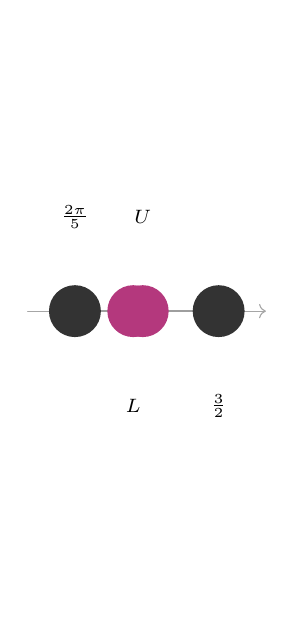
\begin{tikzpicture}[scale=7.500000,line cap=round,line join=round]
\path[use as bounding box] (1.17663706,-0.48000000) rectangle (1.58000000,0.48000000);
\draw[->,black!35] (1.17663706,0)--(1.58000000,0);
\draw[draw=black!38,line width=.7pt] (1.25663706,0.00000000) -- (1.50000000,0.00000000);
\draw[draw=cyan!65!black,line width=.7pt] (1.35547496,0.00000000) -- (1.37141349,0.00000000);
\fill[black!80] (1.25663706,0.00000000) circle (1.25pt);
\fill[magenta!70!black] (1.35547496,0.00000000) circle (1.25pt);
\fill[magenta!70!black] (1.37141349,0.00000000) circle (1.25pt);
\fill[black!80] (1.50000000,0.00000000) circle (1.25pt);
\node[font=\scriptsize,fill=white,inner sep=1.5pt] at (1.25663706,0.16000000) {\(\frac{2 \pi}{5}\)};
\node[font=\scriptsize,fill=white,inner sep=1.5pt] at (1.35547496,-0.16000000) {\(L\)};
\node[font=\scriptsize,fill=white,inner sep=1.5pt] at (1.37141349,0.16000000) {\(U\)};
\node[font=\scriptsize,fill=white,inner sep=1.5pt] at (1.50000000,-0.16000000) {\(\frac{3}{2}\)};
\end{tikzpicture}

\end{center}

\section*{講評}
\noindent\textbf{出題意図}\quad 解析・三角関数の条件を実行可能な関係へ移し、数式を正確に読み取る、計算できる式に直す、初等関数を厳密な上下界で挟むを一つの証明として組み立てる力を問う。

\noindent\textbf{想定する入試}\quad 記述式の大学入試または数学コンテストを想定し、変換の根拠と最終検証までを採点対象とする。

\noindent\textbf{独自性}\quad 数値近似や答えの照合で終えず、問題文から答えまで実際に通過した射と証明義務を再生できる。


\section*{証明の経路}
\begin{center}
\begin{tikzpicture}[
  node distance=3.5mm,
  stage/.style={draw,rounded corners=1pt,align=left,text width=118mm,minimum height=7mm,inner xsep=4pt,inner ysep=2pt,font=\small},
  flow/.style={-{Latex[length=2mm]},thick,cyan!55!black},
  edge label/.style={fill=white,inner xsep=3pt,font=\scriptsize\bfseries}
]
\node[stage] (n0) {問題文};
\node[stage,below=of n0] (n1) {読み取った数式};
\draw[flow] (n0) -- node[edge label] {数式を正確に読み取る} (n1);
\node[stage,below=of n1] (n2) {厳密計算用の式};
\draw[flow] (n1) -- node[edge label] {計算できる式に直す} (n2);
\node[stage,below=of n2] (n3) {初等関数の厳密な上下界};
\draw[flow] (n2) -- node[edge label] {初等関数を厳密な上下界で挟む} (n3);
\node[stage,below=of n3] (n4) {検証済み解答};
\draw[flow] (n3) -- node[edge label] {証明書を再生して結論を認証} (n4);
\end{tikzpicture}
\end{center}

\clearpage
\section*{使った射と役割}
\begin{itemize}
\item \textbf{M1: 数式を正確に読み取る}\\
問題文
$\longrightarrow$
読み取った数式\\
文字、演算、等号、積分区間を区別し、元の数式の構造を保つ。
\item \textbf{M2: 計算できる式に直す}\\
読み取った数式
$\longrightarrow$
厳密計算用の式\\
読み取った数式を、分数や根号を保った厳密計算用の式へ移す。
\item \textbf{M3: 初等関数を厳密な上下界で挟む}\\
厳密計算用の式
$\longrightarrow$
初等関数の厳密な上下界\\
級数の剰余、単調性、積分による順序保存を組み合わせ、浮動小数近似なしで不等式を閉じる。
\item \textbf{M4: 証明書を再生して結論を認証}\\
初等関数の厳密な上下界
$\longrightarrow$
検証済み解答\\
実行記録と証明義務を再生し、元の問題条件に対する結論を確定する。
\end{itemize}




\section*{検証記録}
\begin{itemize}
\item LaTeX数式を構文解析
\item 型付きの実行可能式へ変換
\item 初等関数の厳密な上下界 で厳密計算
\item 未評価演算と制約残差を検査
\item 問題文・解答・検証証明書を出力
\end{itemize}
\noindent\textbf{検証方法}\quad 現在の問題文から合成した証明を、厳密な記号計算と図の根拠から再生
\par\noindent{\footnotesize 証明書 SHA-256: \nolinkurl{afc6a4da0c80ef3080f4f18c311dc2253e24e05222e0a2aed243c4067218e684}}

\end{document}
